\section{Introduction}
\label{sec:introduction}

Dance preparation begins before a visible accent: weight shifts precede a
step, and the body transitions toward a pose before reaching it. A system
dancing to music as it arrives must choose these movements before hearing all
the sound they will accompany. Waiting for an event leaves less time to
prepare; reading the future recording changes the task into offline generation.
Streaming further requires each new movement to continue from an output prefix
that can no longer be revised. Musical anticipation and motion continuation
are therefore coupled requirements of streaming dance generation.

Music-conditioned choreography has advanced through expressive motion models
and large paired datasets~\cite{li2021aist,tseng2023edge,li2023finedance,li2025soulnet}.
Streaming systems such as DiscoForcing~\cite{ji2026discoforcing} encode incoming
audio causally, supporting motion generation as the soundtrack unfolds.
Our question is how to supply prospective musical context when future audio
is unavailable. We investigate this question in robot-native dance: the model
produces reference motion in the humanoid's own configuration space, so musical
choices must be expressed through its body and continued across successive
planning decisions.

\begin{figure*}[t]
\centering
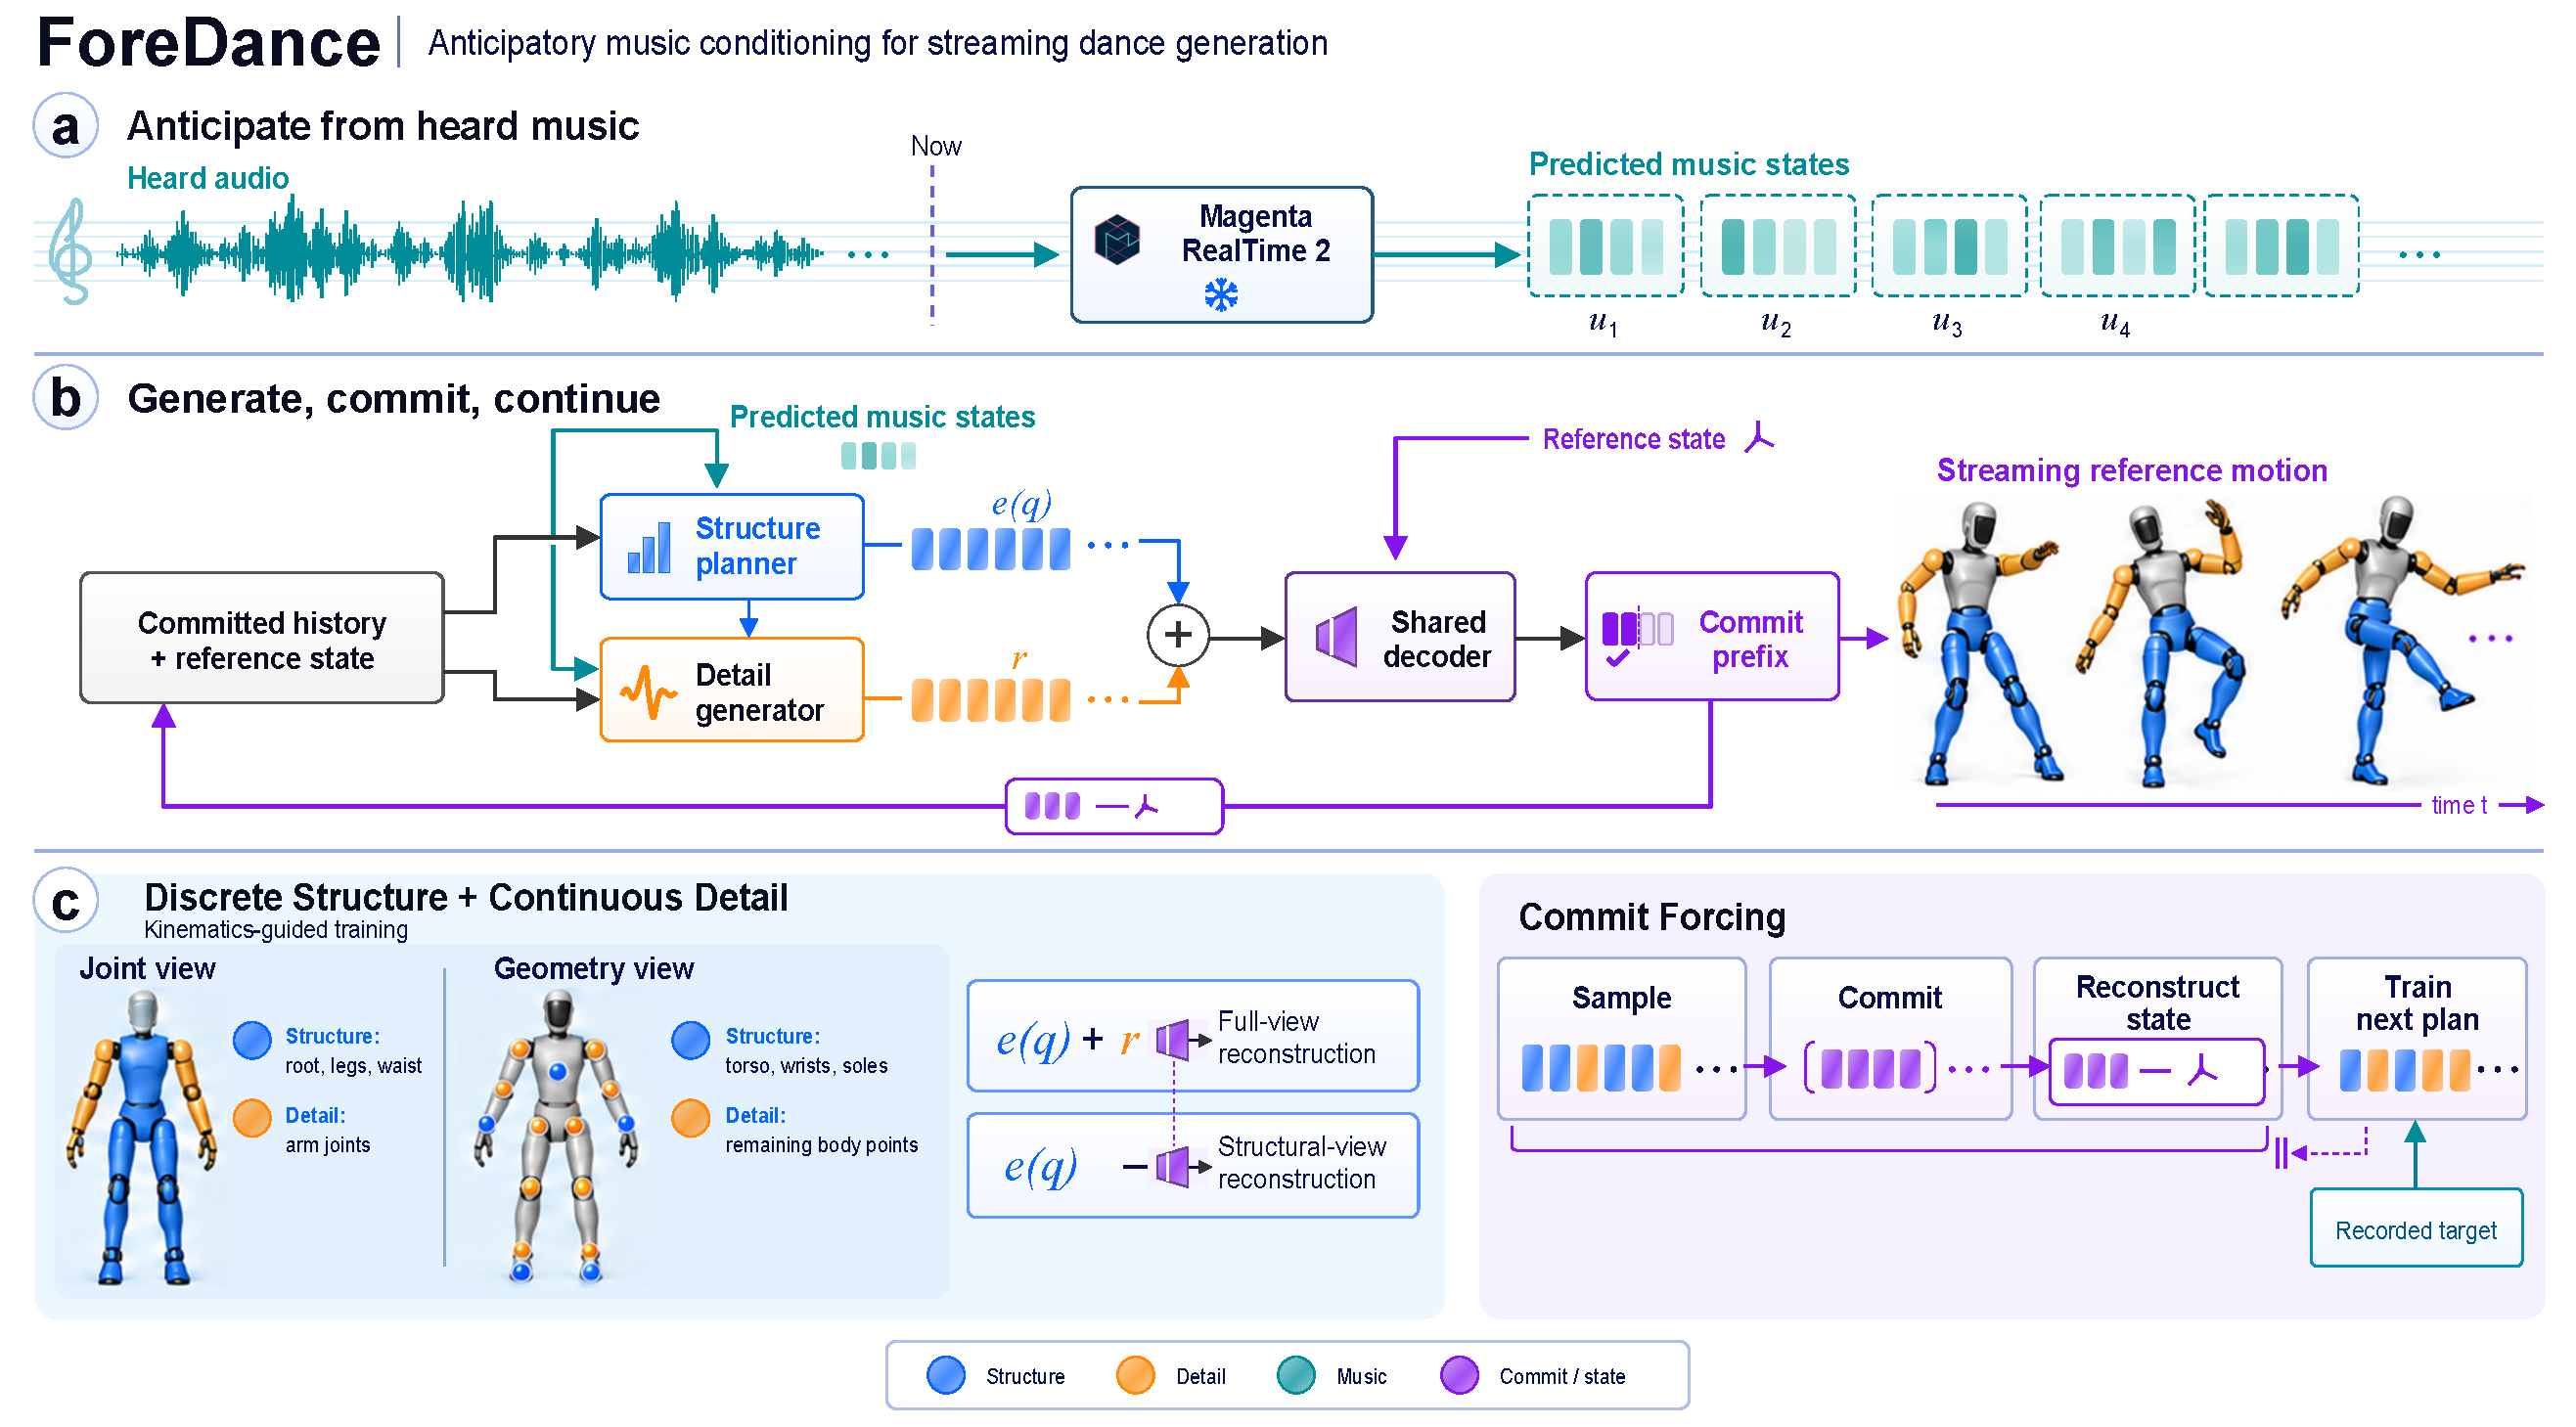
\includegraphics[width=\textwidth]{figures/foredance/overview.pdf}
\caption{\textbf{ForeDance overview.} \textbf{Top:} heard audio supplies a causal forecast of upcoming music states. \textbf{Middle:} the forecast conditions both discrete structure and continuous detail; structure also conditions detail. Their sum passes through a shared decoder, and the committed prefix updates the motion history and reference-derived boundary state for the next decision. \textbf{Bottom:} kinematic supervision gives the two latent components complementary roles, while Commit Forcing trains continuation from a jointly generated history--state pair. Robot poses illustrate the representation and output interface; they are schematic, not experimental or hardware execution evidence.}
\label{fig:overview}
\end{figure*}

We present \method{}, a framework that conditions streaming dance on predicted
future music states. A frozen Magenta RealTime~2 (MRT-2) music foundation
model~\cite{magenta2026mrt2} rolls forward from the audio received so far.
This transfers a general musical continuation prior into dance generation:
paired dance data teaches the motion model to use the prior, while musical
prediction is learned through large-scale music pretraining.
To our knowledge, \method{} is the first streaming dance generation framework
to explicitly condition motion on future music states forecast by a pretrained
music foundation model using past and present audio alone. The predicted
states guide both whole-body organization and complementary articulation.

Realizing this design requires a representation that organizes movement and a
training procedure that accounts for earlier generated choices. Our
kinematics-guided discrete--continuous (D+C) representation couples discrete
structure and continuous detail with complementary reconstruction objectives.
Structure-only reconstruction preserves designated body organization and
endpoint placement; their combination reconstructs full motion through a
shared decoder. Building on hybrid motion representations~\cite{wang2026dcmotion},
this supervision specifies what the two components should preserve.
\cof{} then trains continuation after jointly sampling and committing both
components. Their decoded movement determines the next starting state, pairing
generated history with the reference state it actually induces.

At each decision, \method{} plans a short segment, commits its prefix, and
updates the context for the next plan (Fig.~\ref{fig:overview}). A reference
interface delivers the resulting stream to a fixed SONIC whole-body
controller~\cite{luo2026sonic}. The generator continues from committed references;
measured robot feedback is handled by the controller. This keeps the
motion-generation mechanism explicit while providing a path to motion tracking.

Our contributions are:
\begin{itemize}\setlength{\itemsep}{2pt}
\item \textbf{Anticipatory music conditioning for streaming dance.}
Predicted future states from a frozen music foundation model provide musical
lookahead using arrived audio alone.
\item \textbf{Kinematics-guided D+C representation and paired training.}
Complementary reconstruction objectives establish structural and detail roles
for coupled music-conditioned generation through a shared decoder.
\item \textbf{Commit Forcing for streaming continuation.}
Jointly generated structure and detail define both the committed history and
its resulting reference state for continuation training.
\end{itemize}

We evaluate soundtrack correspondence in 198 generated 60\,s FineDance
trajectories. A frozen G1-native music--motion evaluator favors the intended
soundtrack over alternative gallery tracks in 74.20\% and 75.01\% of pairwise
comparisons under two startup settings, with positive margins in every
training seed. Complementary motion-quality measurements and rendered
references characterize the generated dance. These completed studies establish
correspondence within the framework; Section~\ref{sec:evidence_scope} distinguishes
this evidence from the comparisons needed to attribute forecast and component
benefits.
